\documentclass[12pt,a4paper]{article}

% Paquetes de configuración del documento
\usepackage[utf8]{inputenc}
\usepackage[spanish]{babel}
\usepackage[T1]{fontenc}
\usepackage[margin=2.5cm]{geometry}
\usepackage{fancyhdr}
\usepackage{siunitx}
%Paquetes para simbologia%
\usepackage{amsmath}
\usepackage{amsfonts}
\usepackage{amssymb}
\usepackage{physics}
\usepackage{longtable}
\usepackage{graphicx}
\usepackage{caption}
\usepackage{float}
\usepackage{xurl}
\usepackage[colorlinks=true,
            linkcolor=black,
            urlcolor=myblue,
            citecolor=black,
            filecolor=black]{hyperref}
 % Opción estándar para enlaces
\Urlmuskip=0mu plus 1mu          % Mejora el espaciado para permitir cortes
\usepackage{subcaption}  % en el preámbulo
\usepackage{pgfplots}
\pgfplotsset{compat=1.18}
\usepackage{tikz}
\usepackage{xcolor}
\definecolor{myblue}{RGB}{42, 127, 179}

\pagestyle{fancy}
\chead{\textit{Materiales Metálicos}}
\rhead{\textit{UTN-FRVM}}
\lhead{\textit{Ingeniería Mecánica}}

\begin{document}
\begin{titlepage}
	
	\begin{center}
		{\huge \textit{Universidad Tecnológica Nacional}}\\
        \vspace{0.5cm}
		{\LARGE \textit{Facultad Regional Villa María}}\\
		\vspace{1.5cm}
        {\LARGE{\textit{Ingeniería Mecánica - Materiales Metálicos}}}\\
		\vspace{1.5cm}
        \LARGE{\textit{Trabajo Práctico 3-06}}
	\end{center}
	
	\vfill

    \textit{Grupo DEL RÍO:}
	\begin{itemize}
		\item \textit{Abregú, Iván.}
		\item \textit{Antico, Rodrigo.}
		\item \textit{Brussa,Julián.}
		\item \textit{Cabral, Franco.}
        \item \textit{Cárdenas, Felipe.}
        \item \textit{Cardozo, Martín.}
        \item \textit{Córdoba, Nathan.}
        \item \textit{Cucco, Ramiro.}
        \item \textit{del Río, Juan.}
        \item \textit{Guerini, Nazareno.}
        \item \textit{Medina, Ivo.}
        \item \textit{Ortiz, Gastón.}
        \item \textit{Picos, Elías.}
        \item \textit{Quinteros, Lautaro.}
	\end{itemize}
    
	\textit{Docentes:}
	\begin{itemize}
		\item \textit{Dr. Lucioni, Eldo José.}
		\item \textit{Ing. Victorio Vallaro, Juan Manuel.}
	\end{itemize}
	\centering
	\today
	
\end{titlepage}

\newpage
\tableofcontents

\begin{abstract}
    A partir de la bibliografía listada a continuación, analice e investigue el contenido relacionado con el acero especial indicado por la Cátedra a fin de adquirir la capacidad de explicar el significado de la información que allí se detalla. [REQUERIMIENTO ADICIONAL: Adicionalmente debe investigar si dichos materiales son de uso actual o ha sido reemplazados por otros más modernos.] [NOTA 1: Anualmente la Cátedra asignará los temas a cada equipo de trabajo // NOTA 2: Tenga en cuenta que el requerimiento adicional solo se aplica a la bibliografía indicada. Ver NOTA 3.]
    \begin{itemize}
        \item Apraiz Barreiro, J. Aceros Especiales y Otras Aleaciones. Dossat. 5ta Edición. Madrid, 1975. {MM-CAD-0.0.0}.
        \begin{itemize}
            \item Cap. X Aceros para la fabricación de chapa magnética (pp.221-248) [Caso 2025].
        \end{itemize}
    \end{itemize}
\end{abstract}

\section{Propiedades magnéticas.}
\begin{itemize}
    \item \textbf{Permeabilidad magnética:} facultad que tienen algunos materiales para facilitar el paso a través de ellos del flujo creado por un campo magnético exterior. Es la relación entre la inducción (flujo magnético por unidad de superficie que atraviesa un material) yla intensidad del campo magnético aplicado. Como se aprecia en la \autoref{eq:magnetismo}.
    \begin{equation} \label{eq:magnetismo}
        \mu  = \frac{B}{H}
    \end{equation}
    \item \textbf{Pérdidas por histéresis:} la histéresis magnética es la propiedad que tienen los materiales magnéticos de presentar resistencia al cambio de orientación de sus dipolos magnéticos, al variar la intensidad y el sentido de un campo magnético exterior que actúa sobre ellos. La pérdida de la propiedad ya mencionada representa la energía absorbida por un material bajo la influencia de un campo magnético variable. Se expresa en $Wlb\textsuperscript{-1}$ o \si{\watt\per\kilogram}.
    \item \textbf{Inducción:} flujo magnético por unidad de superficie que atraviesa un material bajo la influencia de un campo magnético exterior, expresado en $\mathrm{gauss}$\footnote{Para ser más prácticos hemos decidido conservar gauss como unidad y no el tesla como dicta el SI para mayor comodidad.}.
    \item \textbf{Saturación:} máximo valor que puede alcanzar lainducción en un material.
    \item \textbf{Modificación Magnética:} variación de propiedades magnéticas que experimentan los materiales con el transcurso del tiempo, por efecto del fenómeno de envejecimiento a temperaturas variables (\SI{20}{\celsius} - \SI{150}{\celsius}). En consecuencia de la existencia de estefenómeno, con el transcurso del tiempo se modifica la microestructura de los materiales, generalmente por precipitación de partículas submicroscópicas en las retículas de los granos aumentando ligeramente su dureza y originando tensiones internas que elevan las  pérdidas magnéticas.
\end{itemize}

En la actualidad, se emplean muchos materiales que se usan en máquinas, instalaciones o aparatos eléctricos, y también son más complejas las características y propiedades que a los mismos se les exigen.
Los aceros o aleaciones que se fabrican especialmente para cumplir especificaciones de carácter eléctrico se pueden clasificar en grupos:

\begin{itemize}
    \item Aceros para la fabricación de chapa magnética.
    \item Aceros o aleaciones de alta permeabilidad.
    \item Aceros o aleaciones magnéticas
    \item Aceros o aleaciones para imanes.
\end{itemize}

De los cuales sólo pondremos el ojo en el primer grupo.

\section{Aceros para la fabricación de chapas magnéticas.}

Se emplean generalmente en forma de chapa o fleje para la fabricación de núcleos o piezas de máquinas eléctricas y transformadores, que están sometidos a la acción de campos magnéticos que cambian rápidamente de valor. Para que tengan un máximo rendimiento, es necesario que las pérdidas de energía organizada por la acción de los campos magnéticos alternativos que actúan sobre ellas sean las más pequeñas posibles.

\subsection{Materiales más usados:}
\begin{itemize}
    \item El material más usado en la actualidad es el acero de bajo carbono (0,25\% - 0,5\%, y con Si 2\% - 4,5\%)
    \item Otros materiales: 
    \begin{itemize}
        \item Hierro dulce de calidad corriente.
        \item Hierro Armco.
        \item Acero moldeado.
        \item Fundiciones.
    \end{itemize}
\end{itemize}

\subsection{Principales propiedades que deben poseer los aceros para chapa magnética.}

Es interesante que este tipo de material tenga alta permeabilidad, y que a su vez las pérdidas por histéresis y pérdidas por corrientes de Foucault, es decir, las pérdidas totales sean pequeñas. También conviene que se pueda laminar sin dificultad, es necesario que tenga buena aptitud al corte (haciendo referencia a una buena maquinabilidad), y por último, que no sea frágil (suficiente resistencia y tenacidad).

\begin{figure}[H]    
    \centering         
    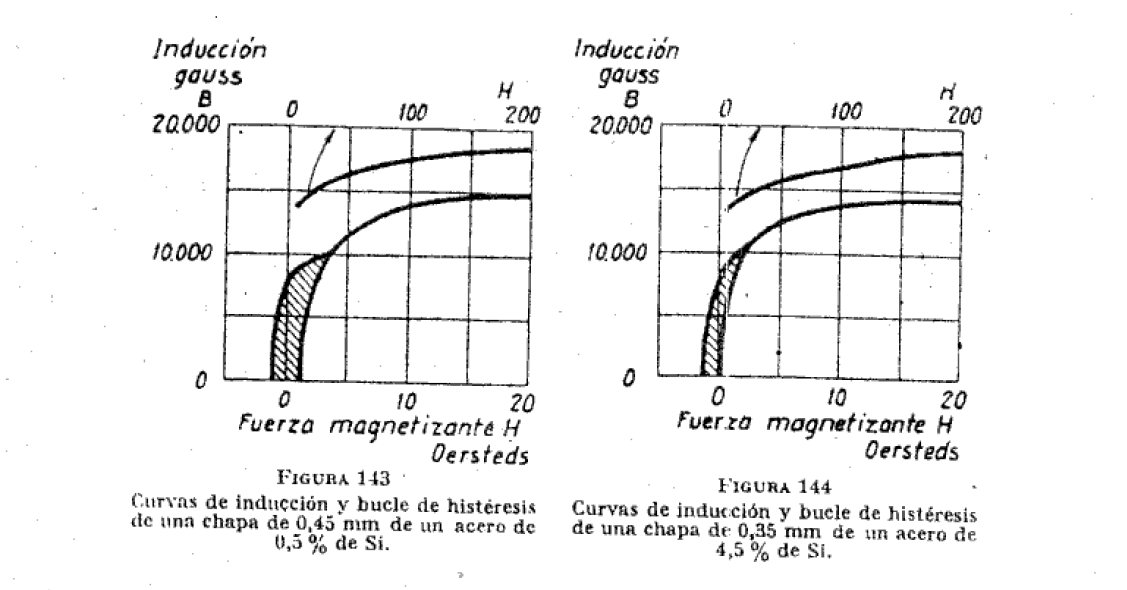
\includegraphics[width=1\textwidth]{IMAGENES LATEX/2.png}
\end{figure}

Las pérdidas por histéresis aumentan al disminuir el tamaño de granos y al aumentar el porcentaje de carbono en los aceros. Por caso contrario, las podemos disminuir si se consigue aumentar la resistividad del acero. Conviene que las chapas tengan el menor espesor posible y que estén bien aisladas unas de otras. En resumen, deben poder las siguientes propiedades:

\begin{itemize}
    \item Pérdidas magnéticas totales pequeñas (para un elevado rendimiento eléctrico).
    \item Elevada permeabilidad magnética (favorecer el paso y concentración del flujo magnético).
    \item Pérdidas por histéresis pequeñas (tamaño de granos grande).
    \item Pequeñas pérdidas por corrientes parásitas o de Foucault (resistividad elevada).
    \item Alto valor de saturación.
    \item No deben sufrir el fenómeno de envejecimiento.
\end{itemize}

\subsection{Evolución de los diferentes tipos de aceros.}

La historia comienza al final del siglo XIX, cuando empezaron a usar láminas de hierro con muy poco contenido de C, éstas tenían unas pérdidas por \SI{5}{\watt\per\kilogram} o \SI{7}{\watt\per\kilogram}. En el año 1900 se empezaron a utilizar hierros extradulces que mejoraron notablemente en la pérdida (\SI{3}{\watt\per\kilogram} a \SI{4}{\watt\per\kilogram}). El inconveniente más grande que tenían estas chapas es que al cabo de unos meses se envejecían y tenías unas pérdidas mucho mayores, pero para el año 1904 se descubrió que el uso de silicio en los aceros mejoraba las propiedades magnéticas, cuando en el 1910 las pérdidas eran de \SI{1,8}{\watt\per\kilogram} y luego de \SI{1,3}{\watt\per\kilogram} para el año 1920. Llegando a 1945 se logró una pérdida de \SI{0,75}{\watt\per\kilogram} con chapas de alta calidad.

Éstas mejoras en las propiedades magnéticas se debe a que el Si tiene alta resistividad eléctrica, y el acero tiene un tamaño de grano relativamente grande debido a la ferrita formada. Sumado a que las chapas de alta calidad no sufren un envejecimiento que sí sufren las chapas de hierros extradulces.

\begin{figure}[H]    
    \centering         
    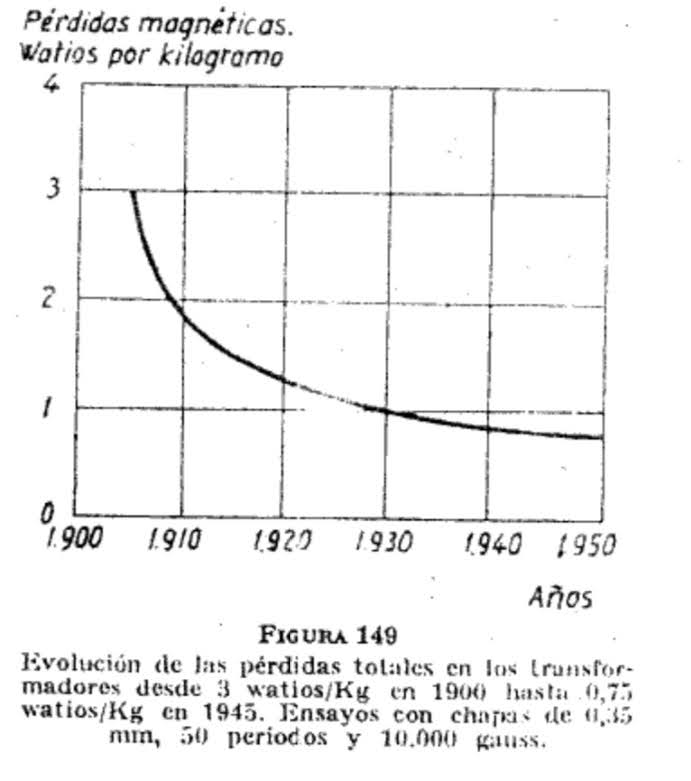
\includegraphics[width=0.5\textwidth]{IMAGENES LATEX/3.jpg}
\end{figure}

\subsection{Modernos estudios sobre chapas magnéticas.}

Algunos factores que más se controlan en la fabricación para chapas magnéticas de las mas alta calidad son: 

\subsubsection{La pureza del material:}

En este caso podemos destacar 5 puntos claves. Entre ellos:

\begin{itemize}
    \item \textbf{Presencia en pequeñas cantidades de carbono, nitrógeno, oxígeno y azufre:} son perjudiciales para las propiedades magnéticas, incluso menos del 0,1\% de C influye en el comportamiento, esta influencia varía según se encuentre en solución sólida o forma de cementita globular, perlita o una solución sobresaturada (martensita).
    \item \textbf{Presencia de azufre y manganeso:}  tienen la misma influencia que el carbono, solo que el azufre actúa más fuerte.
    \item \textbf{Presencia del fósforo:} si esta es mayor al 0,02\% aumenta las pérdidas por histéresis ya que disminuye su permeabilidad.
    \item \textbf{Presencia de elementos endurecedores (cromo, molibdeno,etc):} aunque estos se usan para dar dureza al acero, en esta ocasión son malos para las propiedades magnéticas.
    \item \textbf{Presencia de Gases (hidrógeno, oxígeno, nitrógeno):} si estos están disueltos en el acero no son dañinos pero si estos se encuentran ocluidos (encerrados en burbujas o poros) en el acero si pueden ser perjudiciales.
\end{itemize}

\subsubsection{El tamaño y orientación del grano.}

En este factor encontraremos 3 puntos:
\begin{itemize}
    \item Se sabe que el tamaño y forma del grano influye en las pérdidas magnéticas aunque no todos los investigadores coinciden. En general, que los granos sean más grandes es igual a menos pérdidas por histéresis pero se genera un problema, si los granos son demasiados grandes, aumentan las pérdidas por corriente de foucault, por lo tanto, lo ideal, es regular y controlar el tamaño de grano.
    \item Los pequeños cristales elementales que componen el acero están orientados de forma que las aristas siguen la dirección del flujo, provocando que se necesite menos fuerza para su magnetización. A su vez los cristales cuyas caras forman 45° con la dirección de flujo oponen más resistencia al paso del flujo. En conclusión, la permeabilidad de una chapas con grano orientado es mayor y las pérdidas menores que las chapas con el grano sin orientar.
    \item Mediante el método Goss (obtención de chapas magnéticas con cristales orientados), el cual consiste en someter a la chapas a una serie de laminados en frío con un grado de reducción determinado, seguido de recocidos a determinadas temperaturas con las que se consigue un notable crecimiento del grano. Finalmente se las atraviesa por campos magnéticos orientados en la dirección del laminado se logra un gran aumento de permeabilidad, obteniendo de esta manera aceros de media aleación de silicio, los cuales luego de este procedimiento tienen pérdidas muy bajas, menor fragilidad, mejor ductilidad y fácil laminado. Este tipo de acero es conocido como: “Hipersil” o “High Permeability (HiB)”.
\end{itemize}

\subsubsection{Las tensiones Internas.}
Las tensiones internas con que quedan los materiales, debido a los procesos de laminación o de transformación mecánica, corte o estampación, son muy perjudiciales y deben evitarse por medio de tratamientos de recocidos adecuados, posteriores a todo trabajo mecánico, teniendo cuidado también que los enfriamientos sean suficientemente lentos para que en ellos no nazcan nuevas tensiones.

\subsection{Procesos industriales que se utilizan para la fabricación de chapas magnéticas.}

Se suele obtener en hornos Siemens ácidos empleando chatarras y procesos de trabajo especiales, obteniendo así muy bajos porcentajes de ciertos elementos. En casos menos frecuentes, también se fabrican en hornos Siemens básicos y en hornos de arco eléctrico. Cuando se trata de fabricaciones muy especiales se utilizan también hornos de alta frecuencia con vacío o atmósferas controladas.
Además de para poder orientar los cristales debidamente tenemos que aumentar el tamaño de grano y para eso se suele someter el material al procesos de laminación antes mencionado y a tratamientos térmicos especiales. El proceso se realiza dando primero al material un tratamiento inicial a \SI{750}{\celsius} - \SI{900}{\celsius}, de manera que el acero no llegue a alcanzar el estado austenítico. Luego se suele laminar el material a relativamente baja temperatura (\SI{650}{\celsius} - \SI{800}{\celsius}) no debiendo producirse en el medio una reducción de sección superior al 30\%. Después se da otro tratamiento a temperatura algo más elevada (\SI{800}{\celsius} - \SI{1000}{\celsius}) cuidando también que no se produzca la transformación ferrita-austenita, luego se da el laminado final. A continuación se les da otro tratamiento a \SI{1 000}{\celsius} - \SI{2 000}{\celsius} en atmósfera de hidrógeno o amoníaco disociado con enfriamiento lento hasta los \SI{700}{\celsius} (todos los intervalos de temperatura tienen un sentido en el diagrama de fases, ya que no siempre va haber un cambio de fase a la misma temperatura). En este punto, quedan orientados en el sentido de la laminación de un 25\% - 30\% de los cristales del acero. Luego el montaje en los transformadores debe hacerse de manera que la dirección del flujo magnético sea la misma que la de los cristales.

En la fabricación normal de chapas magnéticas para grandes transformadores es normal realizar recocidos a \SI{800}{\celsius} - \SI{900}{\celsius} en atmósfera de hidrógeno, manteniendo esa temperatura unas 4 a 8 horas según sea el espesor de las chapas y enfriando luego lentamente hasta los \SI{650}{\celsius}.

Para chapas de muy alta calidad se suelen dar recocidos a temperaturas entre \SI{1 000}{\celsius} y \SI{1 200}{\celsius} en atmósferas de hidrógeno seco, enfriando luego lentamente hasta los \SI{850}{\celsius}. En estos recocidos a muy alta temperatura, empleando atmósferas especiales altamente controladas se llega a mejorar la pureza de los aceros, reduciendo los contenidos en C, O y S.

Con frecuencia, posteriormente a estos tratamientos a alta temperatura se les da un recocido oxidante, es decir, calentar un material en una atmósfera de O, generando una capa de óxido en la superficie a \SI{675}{\celsius} para mejorar la permeabilidad.

\section{Aceros al carbono extradulce.}

En este grupo se incluyen los aceros extradulces que se fabrican normalmente con 0,07\% - 0,12\% de C, 0,10 - 0,30\% de Mn y menos de 0,30\% de Si. Usados algunas veces debido a su bajo precio y a su fácil adquisición, a pesar que sus características magnéticas son bastantes bajas. Su máxima permeabilidad (varía según la cantidad de carbono y otras impurezas) es de $1\ 900 \ a \ 5\  000 \ \mathrm{gauss}$ para un campo de $9\ 000 \ \mathrm{gauss}$. La saturación es muy elevada ($21\ 300 \ \mathrm{gauss}$) y la resistividad es de \SI{13e-6}{\Omega}. Por ser la resistividad de estos aceros baja, las pérdidas de Foucault son elevadas, no pudiéndose emplear cuando interesa que las pérdidas sean muy reducidas. Un gran inconveniente de este tipo de acero es que con el tiempo aumentan las pérdidas que tienen inicialmente. Por ser muy sensibles al fenómeno de envejecimiento, pudiendo llegar a duplicar las pérdidas magnéticas después de varios meses de trabajo.

El acero con 0,07\% a 0,12\% de carbono y 0,60\% - 0,90\% de silicio, es decir, con las misma cantidad de carbono que el normal pero con un elevado contenido de Si, tiene mejores propiedades magnéticas que el acero al carbono extradulce ordinario, y puede usarse en algunas máquinas o instalaciones con mejor rendimiento que ellos.

\section{Hierro Armco.}

Aunque el hierro puro es en muchos aspectos un material ferromagnético ideal, ya que su permeabilidad es bastante elevada al resto de materiales, no se puede utilizar para corrientes alternas porque, debido a su baja resistividad, las pérdidas por corriente de Foucault son muy elevadas.

El hierro Armco puede considerarse como el hierro más puro que se obtiene industrialmente en la actualidad y aunque no se fabrica especialmente para utilizarlo en máquinas eléctricas podemos mencionar ciertas propiedades magnéticas que podrían resultar interesante para su utilización en algunos casos determinados.

Se fabrica generalmente en hornos Siemens ácidos y, en general, su contenido en carbono no suele pasar de 0,04\%; el manganeso es inferior a 0,1\%; y el azufre y el fósforo inferiores a 0,02\%. Su máxima permeabilidad es de 6 000 a 8 000 ante un campo de $6\ 000\ \mathrm{gauss}$, al someterlo a tratamientos especiales se reduce el contenido en carbono y otras impurezas elevando de esta manera su permeabilidad a $220\ 000\ \mathrm{gauss}$. La saturación es muy elevada ($21\ 000\ \mathrm{gauss}$) y la resistividad es muy baja (\SI{11e-6}{\Omega}) por esta razón las pérdidas de corrientes Foucault son muy elevadas evitando que se utilice este material para fabricar núcleos para máquinas o aparatos de corriente alterna; lo contrario ocurre con corriente continua; debido a su gran permeabilidad, alta saturación y baja fuerza coercitiva se suele emplear para algunos tipos de dinamos, motores de corriente continua, etc. Incluso con su alta pureza muchas veces se utiliza como materia prima.

El aumento de permeabilidad experimentado al reducir contenidos de impurezas, carbono y otras sustancias el valor es de $7\ 000\ a\ 227\ 000\ \mathrm{gauss}$.

\section{Hierros de gran pureza.}

Aunque se sabía desde tiempos muy antiguos que para la fabricación de chapas magnéticas era conveniente el mayor grado de pureza posible, no fue hasta hace algunos años, que se consiguieron mejoras en las propiedades magnéticas del hierro al reducir el contenido de ciertas impurezas hasta porcentajes más pequeños de lo habitual. Para ello se han realizados ensayos fabricando el acero en hornos de inducción de alta frecuencia, en hornos con atmósfera controlada o fundiendo en vacío y también sometiendo las chapas a recocidos en temperaturas altas (próximas al punto de fusión), en vacío o en atmósferas especiales con hidrógeno seco. 

 \begin{figure}[H]    
    \centering         
    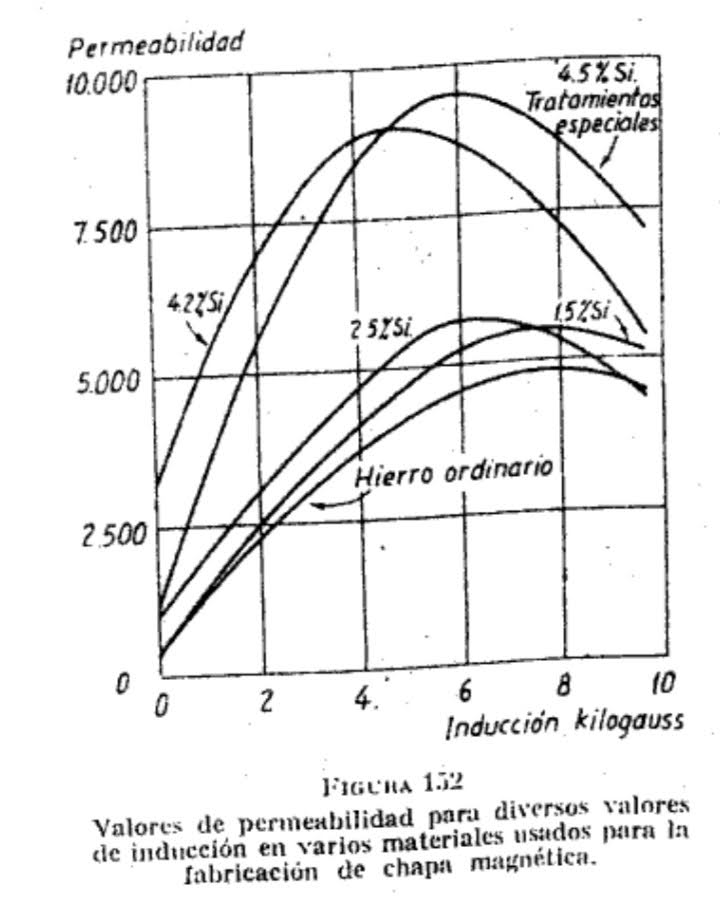
\includegraphics[width=0.5\textwidth]{IMAGENES LATEX/4.jpg}
\end{figure}

%Como se ve, el hierro Armco a pesar de su gran pureza contiene todavía ciertas cantidades de carbono, nitrógeno, azufre y oxígeno, que al situarse en los espacios intersticiales de la retícula cristalina del hierro originan tensiones internas que disminuyen sus propiedades magnéticas. El hierro muy puro tiene además la ventaja de no sufrir el fenómeno de envejecimiento. A la vista de esas características, observando la elevadísima permeabilidad de los hierros muy puros, se comprende que pueda tener en algunos casos aplicaciones de gran interés. Sin embargo, en la actualidad, las dificultades para su fabricación son tan grandes que no se producen industrialmente con normalidad esas calidades, y por lo tanto el empleo de esas clases de pureza muy elevada está casi reducido a ensayos y experiencias de laboratorio.

\section{Fundición.}

Fue bastante usada en los primeros tiempos de la maquinaria eléctrica. Su máxima permeabilidad es muy baja (de $250\ a\ 500\ \mathrm{gauss}$ para un campo de $2\ 000\ a\ 5\ 000\ \mathrm{gauss}$). La saturación también es baja ($14\ 000\ \mathrm{gauss}$) y la resistividad en cambio es muy elevada (\SI{100e-6}{\Omega}). 

Sus características magnéticas son muy bajas, pero por su bajo precio y la facilidad de fundir y mecanizar se emplea todavía en algunas ocasiones en la fabricación de inductores de máquinas de corriente continua.

\section{Acero moldeado.}

Las características magnéticas del acero moldeado (0,1\% - 0,3\% de C) son superiores a las de la fundición. Su máxima permeabilidad (de $700\ a\ 1\ 500\ \mathrm{gauss}$ para un campo de $7\ 000\ \mathrm{gauss}$). Su saturación es muy elevada ($21\ 000\ \mathrm{gauss}$), muy próxima de la del hierro puro. La resistividad es bastante baja (\SI{15e-6}{\Omega}).

\section{Aceros al Si.}

Como vimos en la sección 2.3, a comienzos del siglo pasado, las primeras chapas de acero aleado con silicio se usaban para usos eléctricos que permitieron mejorar notablemente el rendimiento de los transformadores de máquinas eléctricas. El Si y el Al son de los elementos de aleación que más aumentan la resistividad del acero y, como consecuencia, disminuyen extraordinariamente las pérdidas, ya que al ser elevada la resistividad del material hay dificultad para que se produzcan las corrientes inducidas y, por lo tanto, disminuyen las pérdidas por corrientes de Foucault. Cada 1\% de silicio aumenta en 11 microhmios/cm\^2/cm la resistividad de los aceros. El aluminio no se emplea para la fabricación de chapas magnéticas, porque su fabricación presenta dificultades casi insuperables. En los aceros al silicio no se presenta además el fenómeno de envejecimiento tan perjudicial en los aceros al carbono extradulces.

Con un mayor porcentaje a 2,5\% de silicio hace que los aceros sean ferríticos, haciendo referencia a que no se forma austenita al ser calentados a temperaturas altas, favoreciendo a que los granos aumente en los sucesivos calentamientos a los que el el material es sometido reduciendo de esta manera las pérdidas por histéresis.

La permeabilidad no se ha mejorado por la adición de silicio, sigue siendo 6.000 en los aceros de 4,5\% de silicio. Se clasifican en tres grandes grupos según los porcentajes de silicio: 

\begin{itemize}
    \item Alta aleación: 4 a 5\% de silicio.
    \item Media aleación: 2 a 4\% de silicio.
    \item Baja aleación: inferior al 2\% de silicio.
\end{itemize}

Los aceros con alto contenido de silicio son bastantes frágiles, su laminación es difícil y aparecen grietas en los bordes.

\subsection{Características mecánicas:}
Los acero de alto contenido de silicio se emplean exclusivamente en transformadores, en los que las chapas no están expuestas a esfuerzos dinámicos de ninguna clase. En este caso interesa fundamentalmente que las pérdidas magnéticas sean bajas, y en cambio la resistencia o tenacidad del material tiene poca importancia. En los casos donde no son necesarias las más elevadas características magnéticas se prefiere usar aceros de media aleación (de silicio) ya que son de más fácil fabricación y de precio más bajo que los anteriores. En el caso de máquinas rotativas, en las que deben tenerse muy en cuenta las características mecánicas tampoco se emplean los aceros de alta aleación por su gran fragilidad. En las chapas para transformadores interesa, en cambio, que tengan elevadas características magnéticas sin que importen mucho sus propiedades mecánicas, el único requerimiento mecánico que se exige es que se pueda cortar con el troquel sin agrietarse (frecuentemente se suelen calentar las chapas a 100° - 150° para ser cortadas).

\subsection{Factores que modifican los valores de las pérdidas magnéticas.}

Las pérdidas totales de estos aceros son en función:
\begin{itemize}
    \item Del Espesor.
    \item De la Frecuencia.
    \item De la Inducción.
\end{itemize}

\begin{figure}[H]    
    \centering         
    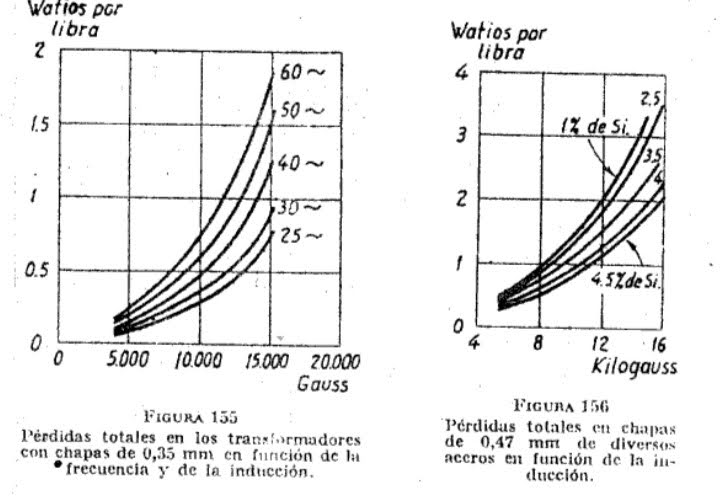
\includegraphics[width=0.6\textwidth]{IMAGENES LATEX/5.jpg}
\end{figure}

\begin{itemize}
    \item Para 10 000 gauss: 
    \begin{itemize}
        \item Chapas de 0,35mm y 4,5\% de silicio: 
        \begin{itemize}
        \item 0,65 watios/libra (con una frecuencia de 60 periodos).
        \item 0.60 watios/libra (con una frecuencia de 50 periodos).
        \item 0,35 watios/libra (con una frecuencia de 30 periodos).
        \item 0,30 watios/libra (con una frecuencia de 25 periodos).
        \end{itemize}
    \end{itemize}
\item Para 5.000 gauss: 
    \begin{itemize}
        \item Chapas de 0,35mm y 4,5\% de silicio:
        \begin{itemize}
            \item 0,20 watios/libra (con una frecuencia de 50 periodos).
        \end{itemize}
    \end{itemize}
\item Para 15.000 gauss:
    \begin{itemize}
        \item Chapas de 0,35mm y 4,5\% de silicio:
        \begin{itemize}
            \item 1,6 watios/libra (con una frecuencia de 50 periodos).
        \end{itemize}
    \end{itemize}
\end{itemize}

Las características más importantes de los aceros al silicio se señalan en la Tabla XXXVI, con los valores de resistividad, saturación y permeabilidad correspondientes a diversos aceros al silicio para chapas magnéticas. En ella podremos observar como las pérdidas disminuyen con el espesor de las chapas y por eso se prefiere usar chapas del menor espesor posibles. Pero como al disminuir el espesor se eleva el precio y aumentan las dificultades de fabricación se han llegado a unos espesores normales:

\begin{itemize}
    \item Para alta aleación: 0,35mm.
    \item Para media aleación: 0,5mm.
    \item Para baja aleación: 0,50 - 1mm
\end{itemize}

\begin{figure}[H]    
    \centering         
    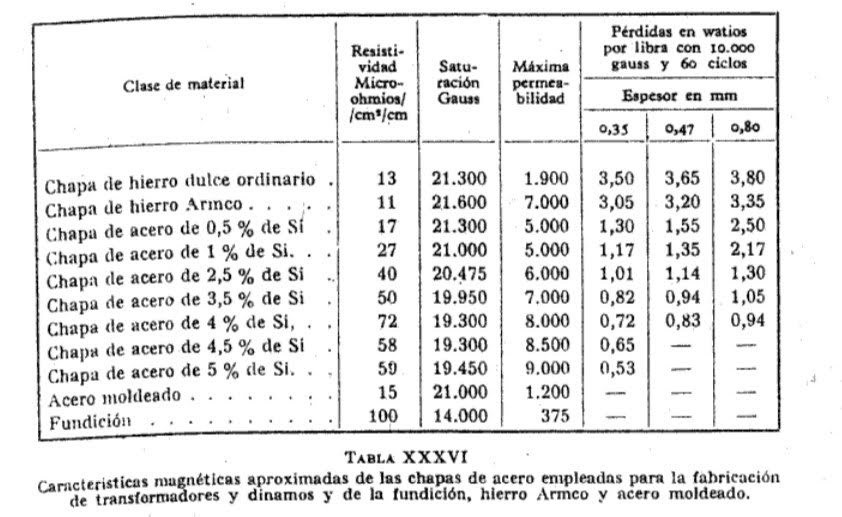
\includegraphics[width=1\textwidth]{IMAGENES LATEX/6.jpg}
\end{figure}

\subsection{Principales aplicaciones de los aceros al Si.}

\begin{itemize}
    \item \textbf{Acero de 0,50\% de silicio:}
    Para pequeños motores de potencia fraccionaria de mediana calidad. Para fabricación de polos estacionarios y otros circuitos que requieren de alta permeabilidad.
    \item \textbf{Aceros de 1\% de silicio:}
    Muy usado para máquinas rotativas, para pequeños motores eléctricos, diferentes tipos de motores y generadores. Para pequeños transformadores de trabajo intermitente, reactores, reguladores de tensión, etc.
    \item \textbf{Acero de 2\% de silicio:}
    Motores y generadores de buen rendimiento, pequeños transformadores, reactancias y otros aparatos donde se admiten pequeñas pérdidas en el núcleo.
    \item \textbf{Acero de 3.5\% de silicio:}
    Motores y generadores de alto rendimiento, transformadores de trabajo intermitente, reactancias y contadores eléctricos.
    \item \textbf{Aceros de 4 - 5\% de silicio:}
    Para fabricación de toda clase de transformadores de alta potencias y motores generadores de alto rendimiento. Transformadores de radio y otras aplicaciones.
\end{itemize}

\section{Aleaciones de alta permeabilidad.}

Hay un grupo de aleaciones de hierro-níquel y otros elementos con 35-80\% de níquel que se caracterizan por su alta permeabilidad y además porque tienen valores de permeabilidad muy elevados cuando se encuentran sometidos a la acción de campos débiles, de baja densidad de flujo. Estás aleaciones son muy utilizadas para cables telefónicos, instrumentos eléctricos, instalaciones de radar, radio, televisión, etc, dónde nos interesa utilizar materiales que posean esas características especiales que acabamos de citar.

Sus pérdidas eléctricas son muy bajas y además las mecánicas de las chapas fabricadas con estás aleaciones son mucho mejores que las chapas con (2 - 4\%) de silicio. Es interesante destacar que estás aleaciones son muy fáciles de laminar aun en perfiles delgados. Pero tienen un inconveniente, ya que se suelen saturar con indicaciones relativamente bajas (8.000 - 12.000 Gauss), además, su alto precio impide su utilización en aparatos baratos de uso corriente, por lo que no sirven todavía para reemplazar los aceros de silicio que tienen un precio más bajo y una saturación de aproximadamente 20.000 Gauss.

Las aleaciones de alta permeabilidad se pueden clasificar en los siguientes grupos:

\begin{itemize}
    \item Aleaciones de alta permeabilidad inicial.
    \item Aleaciones de alto valor de saturación.
    \item Aleaciones de permeabilidad constante.
    \item Aleaciones para realizar compensaciones magnéticas al variar la temperatura (permeabilidad variable con la temperatura).
    \item Aleaciones con variación de dimensiones en la magnetización.
\end{itemize}

\subsection{Aleaciones con muy alta permeabilidad inicial (\textit{Permalloy}, \textit{Permalloy C} y \textit{Supermalloy}).}

Existen una serie de aleaciones de hierro-níquel con 30 - 90\% de níquel que tienen permeabilidades iniciales muy elevadas (10.000 - 100.000) y superiores a la del hierro dulce (250) y a la del acero al silicio (600).

\begin{figure}[H]    
    \centering         
    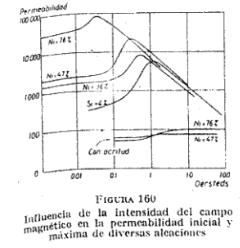
\includegraphics[width=0.5\textwidth]{IMAGENES LATEX/7.png}
\end{figure}

En las con más de 50\% de níquel se consigue mejorar extraordinariamente la permeabilidad inicial por temple al aire, llegando de esa forma a obtener valores elevadísimos. 

Los mejores resultados se obtienen con la aleación de Níquel (78,5\%), que se conoce con el nombre de Permalloy o Permalloy 78,5. La permeabilidad inicial de este, en estado recocido, es de 1.400 aproximadamente, pero después del temple al aire se llega a conseguir una permeabilidad inicial superior a 10.000 y una permeabilidad máxima de 100.000, pero con bajo valor de saturación (11.000 Gauss). Su resistividad eléctrica es aproximadamente (20 x 10\^-6 microhmios por centímetro). Incluso, se han mejorado las características de estás aleaciones adicionando como y molibdeno, obteniendo así: Permalloy-C o Permalloy 79 Mo 4, la cual es una aleación muy representativa de este grupo y con ella se llega a conseguir una permeabilidad inicial de 20.000. Los valores más altos de permeabilidad inicial se alcanzaron con el Supermalloy o Permalloy 79 Mo 5, que después de un tratamiento especial tiene una permeabilidad inicial de 125.000.

La ventaja del empleo de aleaciones con molibdeno es que no es necesario someterlas a ningún tratamiento especial para alcanzar altos valores de permeabilidad inicial.

\subsection{Aleaciones de alta permeabilidad (\textit{Permalloy B Hipernik}).}

Para numerosas aplicaciones en que se desean altos valores de permeabilidad, pero en los que no interesa en cambio que la permeabilidad inicial sea elevada, se pueden emplear aleaciones hierro-níquel con 50\% de níquel, siendo más baratas que las anteriormente mencionadas e inclusive tienen también muy altos valores de permeabilidad.

Son muy utilizadas la aleación Permalloy B o Permalloy 45, que tiene una permeabilidad inicial de 2.700 y una permeabilidad máxima de 23.000. Las características eléctricas de esta aleación se suelen mejorar por recocido a 1.100° en hidrógeno seco. Reduciendo de esta forma el contenido de carbono y azufre, ya que son elementos perjudiciales. La aleación níquel-hierro 50-50 recibe el nombre de Pernik y tiene una permeabilidad inicial de 4.500 y una permeabilidad máxima de 100.000.

\begin{figure}[H]    
    \centering         
    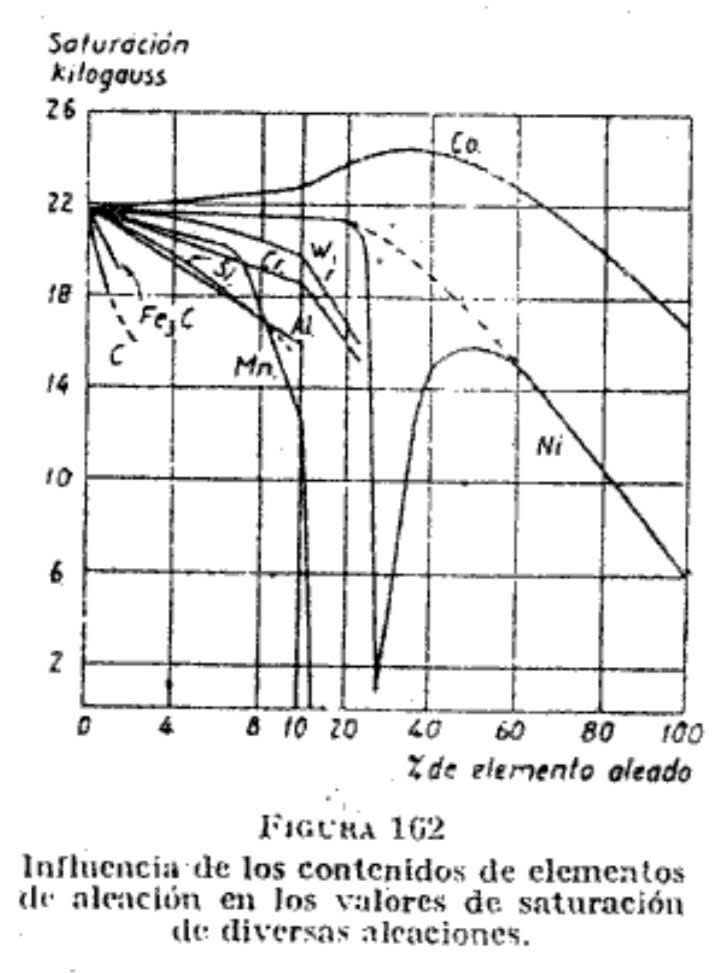
\includegraphics[width=0.5\textwidth]{IMAGENES LATEX/8.jpg}
\end{figure}

\subsection{Aleaciones con alto valor de saturación (\textit{Hiperco} y \textit{Permendur}).}

Para ciertos usos en que interesan valores de saturación se fabrican aleaciones de hierro aleadas con cobalto. Entre todas las aleaciones estudiadas anteriormente, el hierro puro es el que tiene el mayor valor de saturación (21.600). Solo las aleaciones con 0 - 65\% de cobalto tienen valores más elevados.

La aleación Hiperco (Co = 34,5\%), tiene el valor más elevado 24.200. Recibe el nombre de Permendur la aleación (Co = 50\% y Fe= 50\%). Estás aleaciones normalmente no se pueden laminar ni forjar. Pero se ha logrado resolver esta problemática adicionando pequeñas cantidades de cromo y vanadio.

\begin{figure}[H]    
    \centering         
    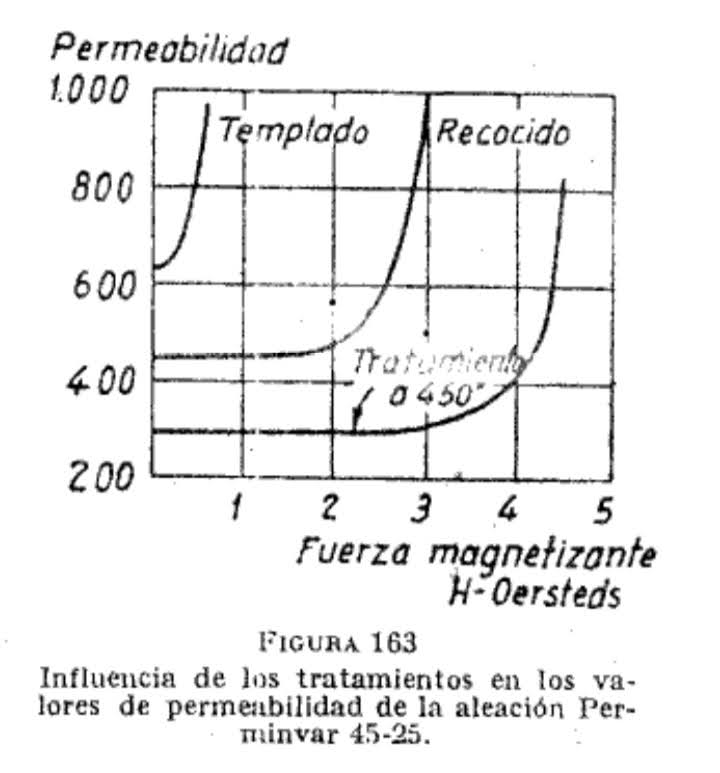
\includegraphics[width=0.5\textwidth]{IMAGENES LATEX/9.jpg}
\end{figure}

\subsection{Aleaciones de permeabilidad constante (\textit{Copernik}, \textit{Isopern} y \textit{Perminvar}).}

La permeabilidad de los materiales magnéticos varía normalmente con la intensidad del campo de imantación que se aplica a cada caso particular. Al ser interesante para numerosas aplicaciones es que el valor de la permeabilidad sea lo más constante posible, incluso a pesar de modificarse el campo de imantación. Para esto se han encontrado materiales (hierro-níquel, hierro-níquel-cobre y hierro-niquel-cobalto) que después de tratamientos especiales poseen esa característica, es decir, permeabilidad casi constante cuando se aplican diferentes intensidades de campo. Los materiales de este grupo en la zona donde el valor de la permeabilidad es constante (bajos valores de inducción) suelen tener valores de permeabilidad bastante bajos (50 - 500).

Dos aleaciones con las que se consiguen permeabilidad constante son el Copernik (las cuales son aleaciones de 40 - 50\% níquel y hierro) y el Isopern (hierro-níquel-cobre), que después de ser sometidas a fuertes reducciones de sección en frío con tratamientos intermedios tienen permeabilidades constantes. A las aleaciones Isopern que contiene 45\% de níquel y 10\% de cobre se les da además un tratamiento de temple desde muy alta temperatura, con lo que se consigue precipitar el cobre. En estás aleaciones se consiguen valores constantes de permeabilidad de 50 - 120.

Otra aleación de este grupo, también muy utilizada, con la que se consiguen permeabilidades constantes bastante elevadas es el Perminvar (níquel-hierro-cobalto) con una composición de 45\% de níquel, 25\% de cobalto y 30\% de hierro. Con esta aleación se consiguen muy buenos resultados al darle un recocido a 900° y luego un calentamiento a 450° durante 24hs con enfriamiento lento. Con este tratamiento y una intensidad magnética (0 - 3 oersted), se consiguen permeabilidades constantes (300) aproximadamente.

\subsection{Aleaciones para realizar compensaciones magnéticas al variar la Temperatura (\textit{Compensator} y \textit{Thermopern}).}

La permeabilidad de los materiales magnéticos disminuye normalmente con la temperatura. Se ha llegado a resolver esta problemática con el empleo de las aleaciones Compensator y Thermopern. Estás son aleaciones que tienen muy bajo el punto de curie (30 - 80°) y por lo tanto cuando se eleva ligeramente la temperatura experimenta una gran pérdida de sus propiedades magnéticas (por transformarse a esas temperaturas el hierro alfa que es magnético en hierro beta amagnético). Para evitar la variación de temperatura modificamos la intensidad del campo que actúa sobre bobinas móviles y otros elementos de los aparatos.

Si se deriva una cierta cantidad del flujo magnético que atraviesa la parte móvil de los aparatos con una pequeña pieza de estás aleaciones con una pequeña pieza de estás aleaciones, al aumentar la temperatura del aparato disminuirá mucho el flujo que pasa por la aleación, lo que ayudará a que se mantenga constante la cantidad de flujo que pasa por la bobina móvil del aparato.

Con ese fin se emplean mucho las aleaciones níquel hierro 30/70 (Compensator). También se emplean aleaciones cobre-níquel (30\% de cobre y 70\% de níquel) denominadas como Thermopern.

\subsection{Aleaciones que experimentan cambios sensibles de volumen al variar la intensidad del Campo Magnético que actúa sobre ella.}

La magnetostricción es una de las muchas propiedades interesantes de las aleaciones hierro-níquel y en especial de las de 50\% de hierro y 50\% de níquel. Estos materiales experimentan un cambio de dimensiones al cambiar la intensidad del campo magnético que los atraviesa. La magnitud del efecto varía con la composición de las aleaciones.

\begin{figure}[t]    
    \centering         
    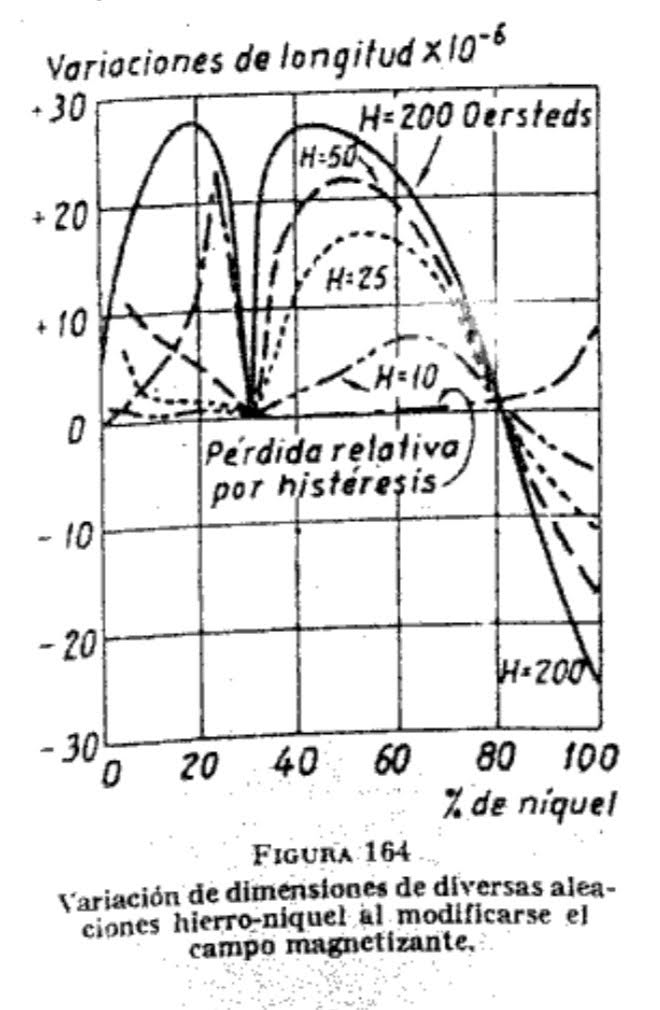
\includegraphics[width=0.5\textwidth]{IMAGENES LATEX/10.jpg}
\end{figure}

Está propiedad se aplica para la transformación de oscilaciones mecánicas en eléctricas y viceversa. La aplicación de un campo eléctrico alternativo en un núcleo magnetostrictivo produce en este una vibración y si las dimensiones del núcleo son adecuadas, se obtiene una resonancia con una apreciable amplitud de oscilación.

Para usos de la marina, por ejemplo, se suelen emplear aleaciones 50\% níquel y 50\% hierro, que además de tener una elevada magnetostricción tienen también una alta permeabilidad y bajas pérdidas por histéresis.

\subsection{Aceros Amagnéticos.}

Para determinadas aplicaciones industriales, interesa emplear materiales metálicos amagnéticos con permeabilidad parecida a la del aire que es la unidad. Para ese fin suelen ser muy empleados metales y aleaciones no férreas, pero en ocasiones en que además es necesario que las piezas tengan elevadas características Mecánicas (gran resistencia, tenacidad, etc) de emplean ciertas aleaciones férreas amagnéticas.

Cuando el hierro es calentado por encima de 768° pasa al estado beta y pierde gran parte de sus propiedades Magnéticas, y al sobrepasar los 910° se transforma en hierro gamma (completamente amagnético).

Se comprende que si fuera posible conseguir con los aceros ordinarios que el estado gamma constituido por cristales de hierro de caras centradas se conservará a la temperatura ambiente estaría resuelto el problema, pero con el empleo de estos aceros esto no sucede así. En la práctica esto solo se puede conseguir con los aceros de alta aleación (austeníticos), en los que la presencia de manganeso, cromo y níquel retardan las transformaciones y por eso es posible obtener aceros austeníticos a temperatura ambiente.

Durante mucho tiempo se ha empleado un acero con 0,25\% de carbono y 25\% de níquel para aplicaciones eléctricas, debido a que es amagnético y posee una buena resistencia mecánica, tenacidad y resistencia a la corrosión. Posteriormente para numerosos usas se han empleado diferentes tipos de aceros austeníticos que no son magnéticos, las clases más utilizadas son: 

\begin{itemize}
    \item Aceros cromo-níquel inoxidable austenítico del tipo 18-8 (18\% cromo y 8\% níquel).
    \item Aceros al manganeso (12\%).
    \item Aceros cromo-níquel de alta aleación austeníticos 14-14 (14\% cromo y 14\% níquel) , 20-12 (20\% cromo y 12\% níquel), y 25-20 (25\% cromo y 20\% níquel).
\end{itemize}

En todos los casos para conseguir mejores resultados conviene someter a las piezas a un tratamiento térmico de austenización que generalmente consiste en calentamiento (1.050° - 1.150°) con enfriamiento al agua, aceite o alcohol aire, según el espesor. Dónde por medio de este tratamiento eliminaremos tensiones residuales y posibles constituyentes (bainita, martensita o aún ferrita, perlita o sorbita) que al ser constituyentes magnéticos reducen las características del material.

\section{Tabla comparativa.}



\begin{figure}[H]    
    \centering         
    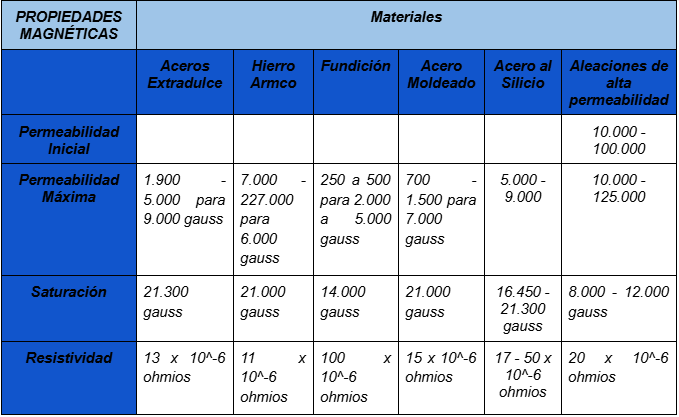
\includegraphics[width=0.88\textwidth]{IMAGENES LATEX/11.png}
\end{figure}

\section{Conclusión.}

En base a nuestra investigación, podemos decir que muchos de los materiales anteriormente mencionados hoy en día se pueden seguir usando, ya que no dejan de ser opciones para la fabricación de chapas magnéticas, si bien la ciencia y tecnología a avanzado siguen siendo buenas alternativas. Por otro lado, hoy en día se está buscando la inversión para ampliar la fabricación de aceros eléctricos al silicio orientados (CRGO). También podemos encontrar materiales como los metales amorfos (vidrio metálico) los cuales tienen estructura cristalina ordenada en las redes y que presentan muy bajas pérdidas por histéresis y corrientes por Foucault.

\end{document}